\documentclass{article}

%% Page Margins %%
\usepackage{geometry}
\geometry{
    top = 0.75in,
    bottom = 0.75in,
    right = 0.75in,
    left = 0.75in,
}

\usepackage{amsmath}
\usepackage{graphicx}
\usepackage{parskip}

\title{Assembly Project: Breakout}

% TODO: Enter your name
\author{Aviraj Newatia}

\begin{document}
\maketitle

\section{Instruction and Summary}

\begin{enumerate}

    \item Which milestones were implemented? 
    % TODO: List the milestone(s) and in the case of 
    %       Milestones 4 & 5, list what features you 
    %       implemented, sorted into easy and hard 
    %       categories.
    \begin{itemize}
    \item   Milestone 1
    \item   Milestone 2
    \item   Milestone 3
    \item   Milestone 4:
    \begin{itemize}
        \item Launching the ball (spacebar)
        \item Pausing the game (p)
        \item Ball Speed Increases on Hit
        \item Restart game at any point, even after losing (r)
    \end{itemize}
    \item Milestone 5:
    \begin{itemize}
        \item Aiming
        \item Multiple-Hit Bricks
        \item Sound on Hitting Brick
    \end{itemize}
    \end{itemize}

    \item How to view the game:
    % TODO: specify the pixes/unit, width and height of 
    %       your game, etc.  NOTE: list these details in
    %       the header of your breakout.asm file too!
    
    \begin{enumerate}

    \item Height 128
    \item Width 64
    \item Height Unit 2
    \item Width Unit 2


    \end{enumerate}

    

\begin{figure}[ht!]
    \centering
    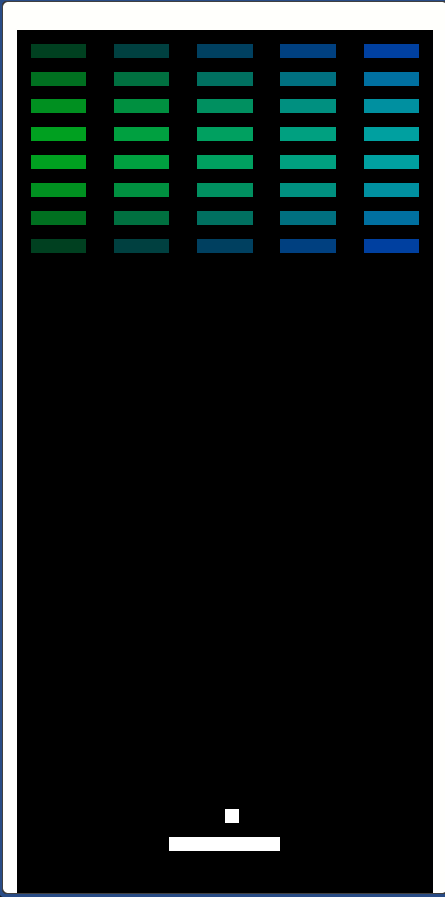
\includegraphics[width=0.3\textwidth]{scene.png}
    \caption{caption}
    \label{Instructions}
\end{figure}

\item Game Summary:
% TODO: Tell us a little about your game.
\begin{itemize}
\item My game plays like a regular breakout at the moment. There's nothing special. Pressing 'q' quits the game.
\end{itemize}

    
\end{enumerate}

\section{Attribution Table}
% TODO: If you worked in partners, tell us who was 
%       responsible for which features. Some reweighting 
%       might be possible in cases where one group member
%       deserves extra credit for the work they put in.

\begin{center}
\begin{tabular}{|| c ||}
\hline
 Student 1 (Aviraj Newatia 1007837708) \\ 
 \hline
 Everything, my nonexistent partner didn't help at all \\ 
 \hline
\end{tabular}
\end{center}

% TODO: Fill out the remainder of the document as you see 
%       fit, including as much detail as you think 
%       necessary to better understand your code. 
%       You can add extra sections and subsections to 
%       help us understand why you deserve marks for 
%       features that were more challenging than they
%       might initially seem.


\end{document}